\documentclass[submission]{dmtcs}

\usepackage[round]{natbib}
\usepackage{graphicx}
\usepackage[latin2]{inputenc}


\usepackage{tikz}%
\usetikzlibrary{arrows,shadows}%
\usepackage{verbatim}%


\usepackage{amsmath}
%\usepackage{cite}
%\usepackage{url}

\newtheorem{definition}{Definition}
\newtheorem{lemma}{Lemma}
\newtheorem{theorem}{Theorem}
\newtheorem{corollary}{Corollary} 

\newcommand{\ZZ}{\mathbb{Z}}
\newcommand{\NN}{\mathbb{N}}
\newcommand{\RR}{\mathbb{R}}

%\newcommand{\comment}[1]{}
\newcommand{\E}[1]{\mathbf{E}\left[#1\right]}

\newcommand{\Beta}[2]{\mathrm{B}(#1,#2)}
\newcommand{\IBETAREG}[3]{\mathrm{I}\left(#1;#2,#3\right)}
\newcommand{\IBETAREGn}[2]{\mathrm{I}\left(\frac1n;#1,#2\right)}

\newcommand{\HarmonicN}[1]{\mathrm{H_{#1}}}

\newcommand{\BigO}[1]{\mathrm{O}\left(#1\right)}
\newcommand{\SmallO}[1]{\mathrm{o}\left(#1\right)}

% komentarze na marginesie
\newcommand{\jci} [1]{\marginpar{\scriptsize {\bf JCi}:#1}}
\newcommand{\MAREK} [1]{\marginpar{\scriptsize {\bf MKlo}:#1}}
\newcommand{\Marek} [1]{\marginpar{\scriptsize {\bf MKlo}:#1}}
\newcommand{\Rafal} [1]{\marginpar{\scriptsize {\bf Rka}:#1}}

\newtheorem{fact}{Fact}
\newtheorem{cor}{Corollary}


\title{
	On the Dynamics of Systems of Urns
%	\thanks{This paper was supported by Polish Ministry of Science and Higher Education --
%	 grant No.  N~N206~1842~33}
}


\author{
	Jacek Cicho\'{n} \and 
	Rafa{\l} Kapelko \and 
	Marek Klonowski
}


\address{
  Institute of Mathematics and Computer Science,\\ 
  Wroc{\l}aw University of Technology, Poland %\\
  %\email{\{Jacek.Cichon, Rafal.Kapelko, Marek.Klonowski\}@pwr.wroc.pl}
}

\begin{document}

\maketitle

\begin{abstract}
In this paper we present an analysis of some generalization of a classic 
urn and balls model. In our model each urn has a fixed capacity 
and balls flow between urns. 
We will show a general form of formulas for the expected numbers of ``black'' balls in a 
given urn and we analyze some special cases (parallel and serial configurations)
We are mainly interested in a counterpart of the Coupon Collector Problem 
for the considered model. 

The primary motivation for our research is the formal analysis of  MIX protocol (introduced by D. Chaum) 
and its immunity against so-called flooding (blending) attacks. 
%Marku, to w co wierzymu nie ma żadnego naukowego znaczenia
%We believe, however, that our results can be applied to 
%analysis of other algorithms as well as some diffusion-like processes.\Marek{Nieco przerobilem %abstract ale dalej mi sie nie podoba}
\end{abstract}


\section{Introduction}

In this paper we investigate following process: we have a finite directed 
acyclic (i.e. without directed cycles) graph  $\mathcal{G} = (V,E)$; we have also a family of urns 
$(U_a)_{a \in V}$ indexed by nodes of  $\mathcal{G}$. 
Each urn contains some number of balls of two kinds - say black and white balls.  
Initially each urn contains only white balls. 
Let us recall that a node $a\in V$ is a source node if there is no $b\in V$
such that $(b,a) \in E$. Similarly, a node $a\in V$ is a sink node 
if there is no $b\in V$ such that $(a,b) \in E$.
At each round (enumerated by natural numbers): 
\begin{enumerate}
\item we choose a random path $v_0,\ldots,v_k$ from source to sink, 
\item we pick randomly balls $b_0, \ldots, b_k$ from urns $U_{v_0}, \ldots, U_{v_k}$, 
\item we remove the ball  $b_k$ from $U_{v_k}$,
\item for each $i<k$ we move the ball $b_i$ to the urn  $U_{v_{i+1}}$,
\item we put one black ball to the urn $U_{v_0}$.
\end{enumerate}
Notice that the number of balls in each urn is constant during the evolution
of this process. We assume that all 
random choices done during the executions of our process are  done independently 
according to uniform distributions.

Notice that if $\mathcal{G} = (\{e\},\emptyset)$ then our model reduces to 
the standard, classical  ``urn model''. 
In our investigations the classical model describes properties of the urns 
indexed by source nodes. The behavior of remaining urns $U_b$ 
depends on the behavior of  of all urns from the family $\{U_a:(a,b) \in E\}$.

The first motivation of our research is the analysis of blending attacks on some kind 
of MIX-es analyzed in e.g. \cite{IH05}, \cite{tic}, \cite{lat}
MIX-es, introduced in the paper \cite{MIX}, are  one of the most popular 
way of protecting anonymous communication. More information about MIX-es can be found in Section~\ref{MIX} 
\Marek{Moze by cos dodac na zasadzie previous work z lini 
badan kul-urn ?}


\subsection{Organization of this paper}

Below we present some basic facts and notation. In Section~\ref{General} we investigate a 
general model. In Section~\ref{Serial} we present a special (however most important for applications)
model wherein urns are assign in a row and balls are consecutively  moved from one urn to another. We present 
several results including some asymptotics. In Section~\ref{Parallel} we investigate 
a system when urns (except a single sink and source) are arrange in parallel. 
We compare some strategies of arranging  urns in Section~\ref{Comparison}. 
In Section~\ref{MIX} we present how our results can be applied to analysis of so-called 
flooding (blending) attack against MIX protocols. 
%We conclude in~\ref{Con}.  


\subsection{Preliminary facts}

In this section we recall some facts about some special function which will be used 
in the analysis in next sections. The partial exponential function $e_n(x)$ is defined 
by the formula
$$
e_n(x) = \sum_{k=0}^{n} \frac{x^k}{k!}.
$$
It is well known (e.g., \cite{WolframFS}) that the sequence $(e_n(n)/e^n)_{n\geq 0}$ is decreasing and

\begin{equation}
\label{expo}
\frac{e_n(n)}{e^n} = \frac12 + \BigO{1/\sqrt{n}}~.
\end{equation}


The Euler Gamma function for $z>0$ is defined by the formula 
$\Gamma(z) = \int_{0}^{\infty} x^{z-1} e^{-x} dx$. For natural numbers $n$ we have
$\Gamma(n+1) = n!$. 
The Euler Beta function is defined for $a,b>0$ by the formula
$\Beta{a}{b} = \int_{0}^{1}x^{a-1}(1-x)^{b-1} dx$. It is well known that 
$\Beta{a}{b} = (\Gamma(a)\Gamma(b))/\Gamma(a+b)$.
The incomplete regularized Beta function is defined by he formula
$$
  \IBETAREG{z}{a}{b} = \frac{1}{\Beta{a}{b}} \int_{0}^{z} x^{a-1}(1-x)^{b-1} dx.
$$
We will use the following two recurrences for incomplete beta function:
\begin{equation}
  \label{icb:rec01}
  \IBETAREG{z}{a}{b} = z \IBETAREG{z}{a-1}{b} + (1-z) \IBETAREG{z}{a}{b-1} ~,
\end{equation}

\begin{equation}
  \label{icb:rec02}
  \IBETAREG{z}{a}{b} = 
  \IBETAREG{z}{a-1}{b} - \frac{\Gamma(a+b-1)}{\Gamma(a)\Gamma(b)} (1-z)^b z^{a-1}~. 
\end{equation}
These formulas may be found in \cite{WolframFS} or \cite{DLMF}). 
They can be also proved by checking that derivatives (taken with respect to the variable $z$)
of both sides of these equations are the same. Clearly, the initial values are the same in both 
sequences.

The incomplete beta function admits an analytical continuation for other values
of parameters. We have, among others, $\IBETAREG{z}{a}{0}=0$ for $a>0$.
 
We denote by $\E{X}$ the expected value of the random variable $X$. Moreover 
if $f(z) = \sum_{i} a_i \cdot z^i$ then $[z^]f(z) = a_i$.  

\section{General Model}\label{General}

Let us fix a finite directed acyclic graph  $\mathcal{G} = (V,E)$.
Let $N=(n_a)_{a\in V}$ denotes capacities of urns $(U_a)_{a\in V}$, 
i.e. $n_a$ is the initial number of white balls in the urn $U_a$.
We call the triple $\mathcal{U} = (V,E,N)$ 
a \textit{system of connected urns}. Note that the number of balls during each process is 
fixed for each urn. Indeed each ball is replaced in each by exactly one. 


\begin{figure*}
\begin{center}
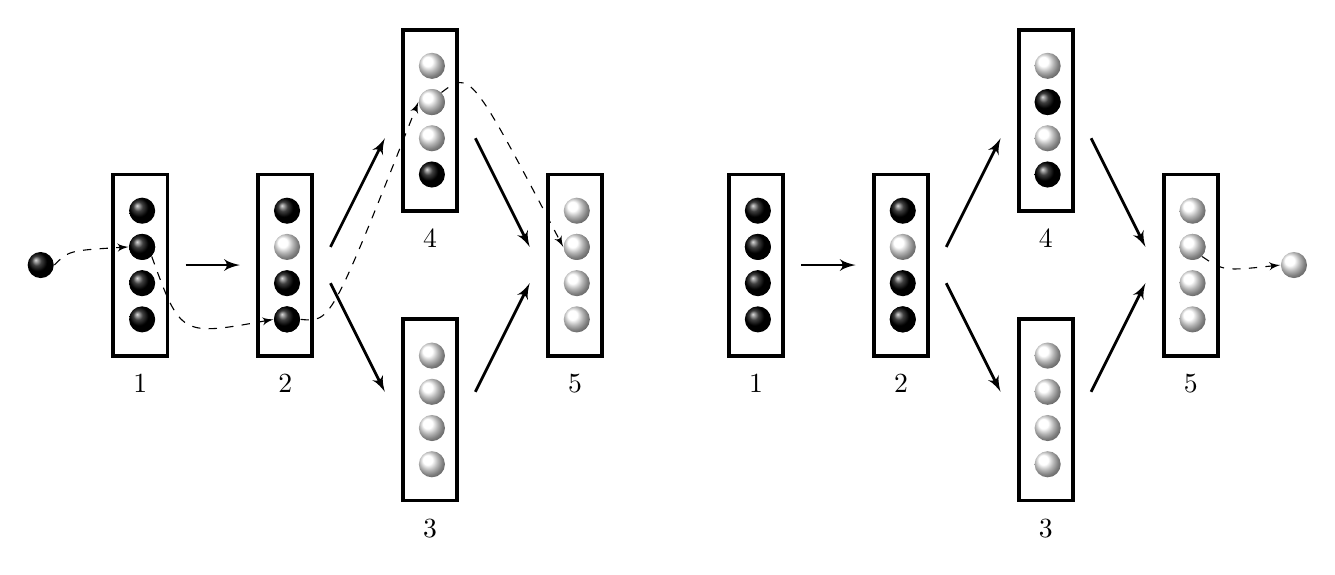
\begin{tikzpicture}[node distance=2.5cm,auto,>=latex',scale=0.92]
        
        \def \rectanglepath#1#2{ -- node (p#1) [below=1mm] {$   #2   $} ++(0.75cm,0cm) -- ++(0cm,2.5cm)  -- ++(-0.75cm,0cm) -- cycle }
        \tikzstyle{bbball}=[circle,shading=ball, ball color=black,  minimum width=0.3cm]
        \tikzstyle{wwball}=[circle,shading=ball, ball color=white,  minimum width=0.3cm]
        \begin{scope}[line width =1.4pt]
        \draw  (0,0) \rectanglepath{1}{1}; % 
        \draw  (2,0) \rectanglepath{2}{2}; %  
        \draw  (4,-2) \rectanglepath{3}{3}; %  
        \draw  (4,2) \rectanglepath{4}{4}; % 
        \draw  (6,0) \rectanglepath{5}{5}; % 
        \end{scope} 
        \begin{scope}[line width =1pt] 
        \draw[->]  (1,1.25) -- (1.75,1.25) ; %
        \draw[->]  (3,1.5) -- (3.75,3) ; %
        \draw[->]  (3,1) -- (3.75,-0.5) ; %  
        \draw[->]  (5,3) -- (5.75,1.5) ; %
        \draw[->]  (5,-0.5) -- (5.75,1) ; %  
        \end{scope}
           
        \foreach \x in {0.5,1,1.5,2}  \node [bbball] at  (0.4,\x) {};  
        \foreach \x in {0.5,1,2}  \node [bbball] at (2.4,\x)  {};
        \foreach \x in {0.5}  \node [bbball] at (4.4,\x +2)  {}; 

        \foreach \x in {1.5}  \node [wwball] at  (2.4,\x) {};  
        \foreach \x in {1,1.5,2}  \node [wwball] at (4.4,\x+2)  {};
        \foreach \x in {0.5,1,1.5,2} \node [wwball] at (4.4,\x -2)  {};
        \foreach \x in {0.5,1,1.5,2}  \node [wwball] at (6.4,\x)  {};        

        \node (p1) [bbball] at (-1,1.25) {};
        \node (p2) [bbball] at (0.4,1.5) {};   
        \node (p3) [bbball] at (2.4,0.5) {};
        \node (p4) [wwball] at (4.4,1.5+2) {};
        \node (p5) [wwball] at (6.4,1.5) {};
         \node (p6)         at (7.8,1.25) {}; 
       

        \draw[dashed,->]  (p1.east) .. controls +(0.2,0.2) .. (p2.west);
        \draw[dashed,->]  (p2.south east) .. controls +(0.4,-1.1) .. (p3.west);
        \draw[dashed,->]  (p3.east) .. controls +(0.42,-0.04) .. (p4.west);
         \draw[dashed,->]  (p4.north east) .. controls +(0.4,+0.3)  ..  (p5.west);
         
%%%%


        \begin{scope}[line width =1.4pt]
        \draw  (8.5,0) \rectanglepath{1x}{1}; % 
        \draw  (10.5,0) \rectanglepath{2x}{2}; %  
        \draw  (12.5,-2) \rectanglepath{3x}{3}; %  
        \draw  (12.5,2) \rectanglepath{4x}{4}; % 
        \draw  (14.5,0) \rectanglepath{5x}{5}; % 
        \end{scope} 
        \begin{scope}[line width =1pt] 
        \draw[->]  (9.5,1.25) -- (10.25,1.25) ; %
        \draw[->]  (11.5,1.5) -- (12.25,3) ; %
        \draw[->]  (11.5,1) -- (12.25,-0.5) ; %  
        \draw[->]  (13.5,3) -- (14.25,1.5) ; %
        \draw[->]  (13.5,-0.5) -- (14.25,1) ; %  
        \end{scope}
           
        \foreach \x in {0.5,1,1.5,2}  \node [bbball] at  (8.9,\x) {};  
        \foreach \x in {0.5,1,2}  \node [bbball] at (10.9,\x)  {};
        \foreach \x in {0.5}  \node [bbball] at (12.9,\x +2)  {}; 

        \foreach \x in {1.5}  \node [wwball] at  (10.9,\x) {};  
        \foreach \x in {1,1.5,2}  \node [wwball] at (12.9,\x+2)  {};
        \foreach \x in {0.5,1,1.5,2} \node [wwball] at (12.9,\x -2)  {};
        \foreach \x in {0.5,1,1.5,2}  \node [wwball] at (14.9,\x)  {};        

        
        \node (p2x) [bbball] at (8.9,1.5) {};   
        \node (p3x) [bbball] at (10.9,0.5) {};
        \node (p4x) [bbball] at (12.9,1.5+2) {};
        \node (p5x) [wwball] at (14.9,1.5) {};
        \node (p6x) [wwball] at (16.3,1.25) {}; 
       

         \draw[dashed,->]  (p5x.south east) .. controls +(0.3,-0.2)  ..  (p6x.west);
         \end{tikzpicture}

\end{center}
  \caption{Example of system of connected urns.  Graph $\mathcal{G}=(\{1,2,3,4,5\},\{(1,2),(2,3),(2,4),(3,5),(4,5)\})$ \label{fig:general} just after round $t=8$ (left side)  and just after round $t=9$ (right side). For each $a\in \{1,2,3,4,5\}$
		we have $n_a=4$. 
		In this picture we have $B_{1}(8)=B_{1}(9)=4$, $B_{4}(9)=W_{4}(9)=2$.}
\end{figure*}



We denote by $p_a$ the probability that randomly chosen path 
from some source to some sink goes through the node $a$. 
If $(a,b) \in E$ then 
we denote by $p_{ab}$ the probability of the event that the edge $(a,b)$ 
is on the randomly chosen path.
Then, if $a$ is a source node then $p_a = \frac{1}{S}$ where $S$ is the 
number of source nodes in the graph $\mathcal{G}$.  
Moreover $p_{ab} = \frac{p_a}{out(a)}$, where 
$out(a) = |\{c\in V: (a,c)\in E\}|$ and
$$
	p_a = \sum \{p_{ba}: (b,a)\in E\}
$$
when $a$ is not a source node. This observation allow us to recursively 
calculate probabilities $p_a$ and $p_{bc}$ for each $a\in V$ and 
$(b,c) \in E$.

Let $B_a(t)$ denotes the number of black balls in the urn $U_a$ 
after the round $t$. Notice that $B_a(0) = 0$ for each $a\in V$.
Our goal is to determine a difference equation for 
the sequence $(\E{B_a(t)})_{t\geq 0}$ for each $a\in V$.

In order to make our considerations more uniform we add one 
artificial node $\bullet$ to our graph and we consider an extended system
with nodes $V_{\bullet}= \{\bullet\} \cup V$, 
edges $E_{\bullet} = E\cup (\{\bullet\}\times S)$ where $S$ is the set of 
source nodes in $(V,E)$
we set capacity
$n_\bullet = 1$ and we put initially one black ball to
the urn $U_\bullet$. Then $B_\bullet(t) = 1$ for each 
$t$ and $p_{\bullet s} = \frac{1}{|S|}$.  
  




Let us fix a node $a \in V$, a round  number $t$ 
and suppose that we know $\E{B_b(t)}$  for each $b\in V$.
Then
\begin{itemize}
\item
At the $(t+1)$th round the number of black urns in the node $a$ may increase by $1$
if there is $b$ such that $(b,a)$ is on the chosen path, 
a black ball was selected from $U_b$ and a white ball was selected from $U_a$.
This happens with probability $p_{ba} \frac{B_b(t)}{n_b} \frac{n_a - B_a(t)}{n_a}$.
\item
At the $(t+1)$th round the number of black urns in the node $a$ may decrease by $1$
if there is $b$ such that $(b,a)$ is on the chosen path, 
a white ball was selected from $U_b$ and a black ball was selected from $U_a$.
This happens with probability $p_{ba} \frac{n_b - B_b(t)}{n_b} \frac{B_a(t)}{n_a}$.
\end{itemize}
Putting this facts together we deduce that
\begin{equation}
\label{eq:generalRecurrence}
\E{B_a(t+1)} = 
\sum_{(b,a)\in E} \frac{p_{b,a}}{n_b} \E{B_b(t)} +
\left(1-\frac{p_a}{n_a}\right) \E{B_a(t)}~.
\end{equation}

Let $W_a(t)$ denotes the number of white balls in the urn $U_a$ 
after the round $t$. Notice that $W_a(t) = n_a - B_a(t)$ for each $a\in V_{\bullet}$, 
so,  among others, we have  $W_{\bullet}(t) = 0$ for each $t$. More generally,
if $d(a)$ denotes the minimal distance of the node $a$ from some 
source link from $V$ then then each $t\leq d(a)$ we have $W_a(t) = n_a$.

After simple transformation we get
\begin{equation}
\label{eq:generalRecurrenceWhite}
\E{W_a(t+1)} = 
\sum_{(b,a)\in E} \frac{p_{b,a}}{n_b} \E{W_b(t)} +
\left(1-\frac{p_a}{n_a}\right) \E{W_a(t)}~.
\end{equation}
Notice that recurrences (\ref{eq:generalRecurrence} ) and 
(\ref{eq:generalRecurrenceWhite}) are the same. 
The solutions of these recurrences
differs on initial conditions.
Let
$$
  F_a(x) = \sum_{t\geq 0} \E{W_a(t)} x^t
$$
be the generating function for the sequence $(\E{W_a(t)})_{t\geq 0}$.
From (\ref{eq:generalRecurrenceWhite}) and from the fact that $F_a(0)=n_a$ we get the following equation 
for each $a\in V$
$$
  F_a(x) = \frac{n_a + x \sum_{(b,a)\in E_{\bullet}} \frac{p_{ba}}{n_b} F_b(x)}{1 - \Delta_a x} ~,
$$
where $\Delta_a = 1 - \frac{p_a}{n_a}$.

Let $prec(a)$ denotes the set of all nodes from $V$ for which there is some oriented path
to the node $a$ (we include the node $a$ in $prec(a)$). For any real number
$x$ and a path $\sigma=(b_1,\ldots,b_n)$ from some source to node $a$ 
we define 
$$
 deg_a(x,\sigma) = |\{k \in \{1,\ldots,n\}:x=\Delta_{b_k}\}| 
$$
and finally we put 
$$
  deg_a(x) = \max\{deg_a(x,\sigma): \sigma \mbox{ is a path from some source to } a\}~.
$$
If $p(t)$ is a polynomial, then by $deg(p)$ we denote the degree of $p$.
We shall formulate a theorem which reduces the problem of finding closed formulas
for $\E{W_a(t)}$ to problems of linear algebra.
This theorem may be treated as a specialized 
form of a theorem about expansion of rational functions 
(see e.g. Theorem IV.9 from \cite{FLA}).

\begin{theorem}
\label{thm:toLineraAlgebra}
Let $a\in V$ and let $D(a) = \{\Delta_b: b \in prec(a)\}$. 
Then there are polynomials
$(p_{\Delta}(t))_{\Delta \in D(a)}$ such that 
$$
	(\forall t\geq 0)\left(
	\E{W_a(t)} = \sum_{\Delta \in D(a)} p_{\Delta}(t) \Delta^t
	\right)
$$
and $deg(p_{\Delta}) < deg_a(\Delta)$ 
for each $\Delta\in D(a)$.
\end{theorem}

\begin{proof}
We claim that for each $a\in V$ there
are polynomials $(\alpha^{a}_{\Delta})_{\Delta \in D(a)}$ and integers 
$(k^{a}_{\Delta})_{\Delta \in D(a)}$ such that 
$deg(\alpha^{a}_{\Delta}) < k^{a}_{\Delta} \leq deg_a(\Delta)$ and
$$
  F_a(x) = \sum_{\Delta\in D(a)} \frac{\alpha^{a}_{\Delta}(x)}{(1-\Delta x)^{k^{a}_{\Delta}}}~.
$$
Observe that if $a$ is a source node then $F_a(x) = \frac{n_a}{1-\Delta_s}$, 
so the claim is true for source nodes.
Suppose hence that the claim is true for all $b\in prec(a) \setminus \{a\}$.
From recurrence (\ref{eq:generalRecurrenceWhite}) we get
$$ 
F_a(x) = \frac{n_a}{1-\Delta_{a} x} +
         \sum_{(b,a)\in E}
				 \sum_{\Delta\in D(b)} \frac{x\cdot\alpha^{b}_{\Delta}(x)}{(1-\Delta x)^{k^{b}_{\Delta}}(1-\Delta_{a} \cdot x)}~.
$$
Let us consider a term
$$
\tau = \frac{x\cdot\alpha(x)}{(1-\Delta x)^{k}(1-\Delta_{a} x)} ~,
$$
where $deg(\alpha)<k$.
If $\Delta_a = \Delta$ then 
$\tau = \frac{x\cdot\alpha(x)}{(1-\Delta x)^{k+1}}$ and
$deg(x\cdot\alpha)< k+1$. If $\Delta_a \neq \Delta$ then we decompose 
$\tau$ into partial fractions and we find a constant B and a polynomial $\beta$ 
such that $deg(\beta)<k$ and
$$
  \tau = \frac{B}{1-\Delta_a} + \frac{\beta(x)}{(1-\Delta x)^{k}}~.
$$
This proves the claim.

Let us fix $\Delta \in D(a)$ and let us consider the term 
$\frac{\alpha(x)}{(1-\Delta)^k}$, where $\alpha(x)$ is some polynomial of degree
less than $k$. Then
$$
  \frac{\alpha(x)}{(1-\Delta)^k} = \sum_{l=0}^{k-1} \alpha_l\frac{x^l}{(1-\Delta)^k}
$$
for some constants $\alpha_0,\ldots,\alpha_{k-1}$.
Observe that
$$
  \frac{x^l}{(1-\Delta)^k} = 
	\sum_{m\geq 0} \binom{m+k-1}{k-1} \Delta^m x^{m+l}~.
$$
Therefore
$$
[x^t]\frac{x^l}{(1-\Delta)^k} =  \Delta^{t-l} \binom{t-l+k-1}{k-1} =
\Delta^{t} \frac{\binom{t-l+k-1}{k-1}}{\Delta^l} =
\Delta^{t} \beta(t)~,
$$
where $\beta$ is a polynomial and $deg(\beta) = k-1$.
Therefore the term $\frac{\alpha(x)}{(1-\Delta)^k}$ is of the same form.
This finishes the proof of theorem.
\end{proof}

Theorem \ref{thm:toLineraAlgebra} gives us a general form of a a solution
of the recurrence equation (\ref{eq:generalRecurrenceWhite}) for a fixed structure
$\mathcal{U} = (V,E,N)$. In order to find required coefficients 
of polynomials $(p_\Delta)_{\Delta\in D}$
we may use the equations 
$W_a(0) = \ldots = W_a(d(a)) = n_a$ and, if $d(a)$ is to small, 
we may solve explicitly the equation (\ref{eq:generalRecurrenceWhite}) for
sufficiently many small values of the time parameter $t$.

%%%%%%%%%%%%%%%%%%%%%%%%%%%%%%%%%%%%%%%%%%%%%%%%%%%%%%%%%%%%%%%%%%%%%%%%%%%%%%
%%%%%%%%%%%%%%%%%%%%%%%%%%%%%%%%%%%%%%%%%%%%%%%%%%%%%%%%%%%%%%%%%%%%%%%%%%%%%%



\section{Serial System of Urns}\label{Serial}

Let us fix two parameters $n$ and $k$.
Let $\mathcal{U}_k = (\{0,\ldots,k\},\{(a,a+1):a<k\},N)$.
where $n_a = n$ for each $a \in \{0,\ldots,k\}$. That is, each urn has the same capacity.
Therefore at each round we move one ball from urn $U_a$ to $U_{a+1}$ (if $a<k$), we remove
one ball from $k$th urn and we add one black urn to the urn $U_0$.
As before, we assume that we choose the balls independently, using uniform distributions.
Note that this model strictly corresponds to so-called \textit{mix-cascade} described in Section \ref{MIX}. 

The evolution of this model is described by the vector 
$B(t) = (B_0(t),\ldots,B_k(t))$
of black balls in consecutive urns. Notice that $B(0) = (0,\ldots,0)$.
Let us observe that the random variable $B_0$ describes the 
classic urn and balls problem and $\E{B_0(t)} = n\left(1- \left(1-\frac1n\right)^t\right)$.
Clearly $B_0(0)\leq B_0(1) \leq B_0(2)\leq \ldots$. 
But if $k>0$ then the processes $(B_a(t))_{t\geq 0}$ are not monotonic with probability $1$ - 
for example $\Pr[B_1(2)=1, B_1(3)=0] = \frac{n-1}{n^3} > 0$.



\subsection{Difference equations}

Since we are going to analyze behavior of the system $\mathcal{U}_k$
for arbitrary $k$ instead of using Theorem \ref{thm:toLineraAlgebra} 
we shall solve directly the recurrence \ref{eq:generalRecurrence} 
adopted to this case.
Notice that for each $a\in\{0,\ldots,k\}$ we have $p_a=1$ and that 
$p_{a,a+1} = 1$ for each $a=0,\ldots,k-1$. 

For  $a \in \{1,\ldots,k\}$ we obtain from Equation \ref{eq:generalRecurrence}
the following recurrence: 
\begin{equation}
\label{eq:Ya}
    \E{B_{a}(t+1)} = \frac{1}{n} \E{B_{a-1}(t)} +(1-\frac{1}{n}) \E{B_{a}(t)}.
\end{equation}

Let $y_a(t) = \E{B_{a}(t)}$, $\delta=\frac{1}{n}$ and $\Delta = 1 - \frac{1}{n}$. 
Then the initial observation and the equation (\ref{eq:Ya}) can be rewritten as

\begin{equation}
\label{eq:all}
\left\{
\begin{array}{rcl}
y_{0}(t)     &=& n (1 - \Delta^t)\\
y_{a+1}(t+1) &=& \Delta\cdot y_{a+1}(t) + \delta\cdot y_{a}(t)~.
\end{array}
\right.
\end{equation}
%
Let us also recall that $y_{a}(0)=0$ for each $a$.
It is also clear  that $y_{a}(t)=0$ for each $t\leq a$.


\subsection{Closed formula}

We will show in this section that there exists a closed formula for
the expected value of the random variable $B_{a}(t)$ for arbitrary $a$ and $t$.

\begin{theorem} 
\label{thm:IBF}
For each $a\geq 0$ and $t\geq 0$ we have
$$
  \E{B_{a}(a+t)} = n \cdot \IBETAREGn{a+1}{t} ~.
$$
\end{theorem}

\begin{proof}
Let $z_a(t) = y_a(a+t)$ and $\Delta = 1 - \frac1n$ and $\delta = \frac1n$.
Note that $z_{a}(0) = 0$ for each $a$, 
$z_{0}(t) =  n(1 - \Delta^t)$ and
\begin{gather*}
z_{a+1}(t+1) = y_{a+1}((a+t+1)+1) =
\Delta \cdot y_{a+1}(a+1+t)  + \delta \cdot y_{a}(a+t+1) = \\
\Delta\cdot z_{a+1}(t) + \delta\cdot z_{a}(t+1)~.
\end{gather*}

Therefore the equations (\ref{eq:all}) may be rewritten
as follows:
\begin{equation}
\label{eq:allX}
\left\{
\begin{array}{rcl}
z_{0}(t)   &=& n(1 - \Delta^t)\\
z_{a+1}(t+1) &=& \Delta\cdot z_{a+1}(t) + \delta\cdot z_{a}(t+1)~.
\end{array}
\right. ~,
\end{equation}

A direct calculus shows that
$$
n \cdot \IBETAREGn{1}{t} =  n \frac{\Gamma(t+1)}{\Gamma(1)\Gamma(t)} \int_{0}^{\frac1n} (1-x)^{t-1} dx = 
n \left(1- \left(1-\frac1n\right)^t\right) ~,
$$
so $z_0(t) = n \IBETAREGn{1}{t}$.
From equation (\ref{icb:rec01}) applied for $z=\frac1n$
we get 
\begin{equation}
   n \cdot \IBETAREGn{a+2}{t+1} = 
   \Delta \cdot n \cdot \IBETAREGn{a+2}{t} +\delta\cdot n \cdot \IBETAREGn{a+1}{t+1} ~.
\end{equation}
Moreover  $n \cdot \IBETAREGn{a+1}{0} = 0$
therefore the sequences $(z_a(t))_{a,t}$ and $(n \IBETAREGn{a+1}{t})_{a,t}$ 
satisfy the same recurrence relations.
\end{proof}

%\begin{figure}[!t]
  %\begin{center}
     %\includegraphics[width=0.75\textwidth]{ExpectedValues.pdf}
  %\end{center}
  %\caption{Graphs of $\E{B_{a}(t)}$ for $n=1000$ and $a=0\ldots 7$}
  %\label{fig:5mixerow}
%\end{figure}


Theorem \ref{thm:IBF} gives us a closed formula for the 
expected number of black balls after a given number of steps in a given urn.
However, we will need an another formula for 
$\E{B_{a}(a+t+1)}$ which we found convenient for investigation of 
properties of a fixed urn and for various values of $t$. 

\begin{theorem}
\label{thm:goodformula}
\begin{equation}
\label{eq:ya}
  \E{B_{a}(a+t+1)} =  
  n\left(1- \left(1-\frac{1}{n}\right)^{t+1} \sum_{k=0}^{a} \binom{k+t}{k}\frac{1}{n^k}\right)~.
  \end{equation}
\end{theorem} 

\begin{proof}
From formula (\ref{icb:rec02}) we deduce that
$$
  \IBETAREG{z}{a+1}{t+1} = 
	\IBETAREG{z}{a}{t+1} - \binom{a+t}{a} (1-z)^{t+1} z^a ~.
$$
Moreover, we know that 
$$
\IBETAREG{z}{1}{t+1}  = 1 - (1-z)^{t+1} = 
  1 - \binom{0+t}{0} (1-z)^{t+1} z^0
$$
so we get
$$
  \IBETAREG{z}{a+1}{t+1} = 1 - 
	\sum_{k=0}^{a} \binom{k+t}{k}(1-z)^{t+1}z^k~.
$$
After putting $z= \frac1n$ into this formula and using Theorem \ref{thm:IBF}
we get desired identity.
\end{proof}

%\begin{proof}
%We know that $\E{Y_{0}(0+t+1)} = n(1-(1-\frac1n)^{t+1})$.
%From formula (\ref{icb:rec02}) we deduce that
%\begin{gather*}
%\E{Y_a(a+t+1)} = n \IBETAREGn{a+1}{t+1} = \\
%n\left(\IBETAREGn{a}{t+1} -  
%\frac{\Gamma(a+t+1)}{\Gamma(a+1)\Gamma(t+1)}(1-\frac1n)^{t+1}\frac{1}{n^a}
%\right) = 
%\\
 %\E{Y_{a-1}((a-1)+t+1)} - \binom{a+t}{a} (1-\frac1n)^{t+1}\frac{1}{n^a}~, 
%\end{gather*}
%from which we get the required equation.
%\end{proof}

\subsection{Asymptotic behavior}

In this section we investigate asymptotic behavior of the system of urns. 
In particular it is important for us, when the first black ball appears in particular 
urn, when the fixed urn is full of black balls and when a big portion of balls in a given
urn is black.  

%The behavior of the random variable $Y_0$ is well--known. Among other
%we have $Y_0(0) = 0$, $Y_0(1) = 1$, $\E{Y_0(n \ln 2)} = \frac12 n + \BigO{1}$ and
%$\E{Y_n(n \ln n)} = n - 1 +\BigO{\frac{\ln n}{n}}$. 
%Moreover $Y_0(0)\leq Y_0(1) \leq Y_0(2)\leq \ldots$.

\subsubsection{When almost all balls are black ?}

We shall investigate in this section the moment at which almost all
balls in given layer are black. More precisely, we fix the number $n$ of balls 
in each layer and we want to approximate the moment when $n-1$ balls in 
a given urn are black.

\begin{lemma}
\label{xxx2}
Let $t_n = n(\ln(n) + (a + \nu )\ln(\ln(n)) - \ln(a!))$ for some $\nu \geq 0$.
If $0\leq k < a + \nu$ then
$$
 n\left(1-\frac1n\right)^{t_n} \binom{k+t_n}{k}\frac{1}{n^k} = 
 \BigO{\frac{1}{(\ln n)^{a + \nu -k}}}~.
$$
and for $k=a$ and $\nu=0$ we have
$$
 n\left(1-\frac1n\right)^{t_n} \binom{a+t_n}{k}\frac{1}{n^a} = 
 1 + \BigO{\frac{\ln\ln n}{\ln n}}~,
$$
\end{lemma}

The proof of this lemma can be instantly deduced from the following
equation
%\begin{proof}
%Let us observe that
\begin{equation}
\label{lll:1}
\ln \left(1-\frac1n\right)^{t_n} = 
  - t_n \ln\frac{1}{1-\frac1n} = 
 - \frac{t_n}{n}\left(1+\BigO{\frac1n}\right)~.
\end{equation}
%from which we easily deduce that
%\begin{gather*}
%\left(1-\frac1n\right)^{t_n} = 
  %\frac{a!}{n (\ln n)^{a+\nu}} \left(1 + \BigO{\frac{\ln n}{n}}\right)~.
%\end{gather*}
%
%Let us consider any number $k \leq a$. The we have
%\begin{gather*}
%\binom{k+t}{k}\frac{1}{n^k} = 
%\prod_{j=0}^{k-1}(t+k -j) \frac{1}{k! \cdot n^k} =
%\frac{1}{k!} \left(\frac{t}{n}\right)^k \prod_{j=1}^{k}\left(1+\frac{j}{t}\right)  
%\end{gather*}
%hence
%\begin{gather*}
%n\left(1-\frac1n\right)^{t_n} \binom{k+t_n}{k}\frac{1}{n^k} =
%\frac{a!}{k!} \left(\log n\right)^{k-\nu-a} \left(1 + \BigO{\frac{\ln\ln n}{\ln n}}\right)~.
%\end{gather*}
%\end{proof}


\begin{theorem}\label{thm4xc}
If  $a$ is fixed and $t_n = n(\ln(n) + a \ln(\ln(n)) - \ln(a!))$ then
$$
\E{B_{a}(a+t_n)} = n-1 + \BigO{\frac{\ln\ln n}{\ln n}}~
$$
as $n$ approach infinity.
\end{theorem}

\begin{proof}
The theorem is a consequence of Lemma~\ref{xxx2} (with $\nu=0$) and 
Theorem \ref{thm:goodformula}.
\end{proof}

Notice that for $a=0$ we get 
$\E{B_{0}(n\ln n)} = n-1 + \SmallO{n}$,
so our result is consistent with the classical Coupon Collector Problem 
(see \cite{Feller1}). We shall come back to this problem in 
Sec. \ref{sec:FinalRemarks}.
Below we show that just after the time 
$n(\ln n + \ln ((\ln n)^a/a!))$
all balls in $a$th urn are black with high probability.

\begin{theorem}\label{thm5xc}
If  $a$ and $\nu>0$ are fixed and $t_n = n(\ln(n) + (a+\nu) \ln(\ln(n)) - \ln(a!))$ then
$$
\Pr[B_{a}(a+t_n)\neq n] = \BigO{\frac{1}{(\ln n)^{\nu}}} ~.
$$
as $n$ approach infinity.
\end{theorem}

\begin{proof}
Notice that the number of white balls in the $t_n$-th round in the $a$-th urn is
$W_a(t_n)=n-B_{a}(a+t_n)$. Thus $W_a(t_n)\neq 0$ is equivalent to
$B_{a}(a+t_n)\neq n$. However $\Pr[W_a(t_n)\neq 0]\leq \E{W_a(t_n)} 
= n - \E{B_{a}(a+t_n)}$ as $W_a(t_n)$ is integer valued, non-negative random variable.  
Thus, to prove our theorem it is sufficient  
to show that $\E{B_{a}(a+t_n)} = n - \BigO{\frac{1}{(\ln n)^{\nu}}}$. 
This is however the consequence of Lemma~\ref{xxx2} with $\nu > 0$ and  
Theorem \ref{thm:goodformula}~.
\end{proof}
\Marek{Uwaga, zmienione oznaczenia !}


\subsubsection{First black ball}

Let us recall that $B_0(1) = 1$. For arbitrary $a$ we have the 

\begin{theorem}
\label{thm:first}
If $a$ is fixed and $t_n = ((a+1)! n^a)^{\frac{1}{a+1}}$ then
$$
\lim_{n\to\infty} \E{B_{a}(a+t_n)} = 1~.
$$
\end{theorem}

\begin{proof} 
Let us observe that for all $x \in [0,\frac{1}{n}]$ we have
$x^a (1-\frac{1}{n})^t \leq x^a(1-x)^{t-1} \leq x^a$, 
hence
$$
  \frac{n}{\Beta{a+1}{t}}(1-\frac{1}{n})^{t-1} \int_{0}^{\frac1n}x^a dx \leq
  n \IBETAREGn{a+1}{t}
$$
and
$$
  n \IBETAREGn{a+1}{t} \leq
  \frac{n}{\Beta{a+1}{t}} \int_{0}^{\frac1n}x^a dx ~,
$$
so
$$
\frac{\Gamma(a+t+1)}{\Gamma(t)} (1-\frac{1}{n})^{t-1} \frac{1}{(a+1)!n^a} \leq
n \IBETAREGn{a+1}{t} \leq
\frac{\Gamma(a+t+1)}{\Gamma(t)} \frac{1}{(a+1)!n^a} ~.
$$
Notice that
$$
\frac{\Gamma(a+t+1)}{\Gamma(t)} = t^{a+1} \prod_{j=0}^{a}(1+\frac{j}{t})~,
$$
so 
$$
 \frac{\Gamma(a+t_n+1)}{\Gamma(t_n)} = 
 (a+1)!\cdot n^{a}\left(1+ \BigO{\frac{1}{n}}^{\frac{a+1}{a}}\right)~.
$$
Moreover from equation (\ref{lll:1}) we get
$$
\left(1-\frac1n\right)^{t_n}  = 1 + \BigO{\frac1n}^{\frac{1}{a+1}}~,
$$
so the proof is finished.
\end{proof}

If we apply Theorem \ref{thm:first} to $a=1$ then we get
$\E{B_1(1+\sqrt{2n})} \approx 1$, so we see that the first moment when the first 
black urn appears in the urn $U_1$ is closely related with expected number $T_n$
of steps when the classical Birthday Paradox occurs (let us recall that 
$T_n = \sqrt{\pi n/2} + \BigO{1}$).

\subsubsection{Near half balls are black}

Let us recall that $e_a(a)/{e^a}$ is close to $\frac12$ (see Eq. (\ref{expo})). 
We will show in this section that at time $an$ nearly half of balls 
in $a$th urn are the back.

\begin{theorem}\label{thm7xc}
If $a$ is fixed and $t_n = a\cdot n$ then
$$
  \E{B_{a}(a+t_n+1)} = n\left(1-\frac{e_a(a)}{e^a}\right) + \BigO{1}.
$$
\end{theorem}


\begin{proof}

Let us note that applying equation~\ref{lll:1} we can easily prove that 

$$(1-\frac1n)^{an+1} = e^{-a}(1+\BigO{\frac1n})~.$$

Moreover
\begin{gather*}
\binom{k+a n}{k} = \frac{1}{k!} \prod_{j=0}^{k-1} (k+an-j) = 
\frac{a^k n^k}{k!} \prod_{l=1}^{k} (1+\frac{l}{a n}) =
\frac{a^k n^k}{k!}(1+\BigO{\frac1n})~.
\end{gather*}
Therefore
$$
(1-\frac1n)^{an+1} \binom{k+a n}{k} \frac{1}{n^k} = 
e^{-a} \frac{a^k}{k!}(1+\BigO{\frac1n})~.
$$
From Theorem \ref{thm:goodformula} we get
\begin{gather*}
 \E{Y_a(a+an+1)} = 
 n\left(1 - \sum_{k=0}^{a} e^{-a} \frac{a^k}{k!}(1+\BigO{\frac1n})\right) = \\
 n\left(1 - e^{-a} (\sum_{k=0}^{a} \frac{a^k}{k!}) (1+\BigO{\frac1n})\right) = 
 n\left(1 - \frac{e_a(a)}{e^a} (1+\BigO{\frac1n})\right) = \\
 n\left(1 - \frac{e_a(a)}{e^a} + \BigO{\frac1n}\right) =
 n\left(1 - \frac{e_a(a)}{e^a}\right) + \BigO{1}~,
\end{gather*}
so the theorem is proved.
\end{proof}




\section{Parallel system of urns}\label{Parallel}

In the previous section we investigate a serial system of urns.
In this section we consider an another variant of system,
namely, let $\mathcal{G} = (\{0,\ldots,k+1\},E)$, where
$E= (\{0\}\times\{1,\ldots,k\}) \cup (\{1,\ldots,k\}\times\{k+1\})$.
We assume, as before, that the capacity of all urns is $n$ and that at the 
beginning of considered process all balls are white.

At each step we select one path $0 \to i \to (k+1)$ where $i \in \{1,\ldots,k\}$ 
with the same probability, next we choose balls from selected urns, we move balls according 
to arrows and put a black ball in the selected place in the urn $U_0$.
Observe that $p_0=p_{k+1}=1$, $p_{0a} = \frac1k$, $p_{a(k+1)} = 1$ and 
$p_a  = \frac1k$ for each  $a \in \{1,\ldots,k\}$.

Let $W_{k+1}(t)$ denotes the number of white balls in the urn $U_{k+1}$ 
after $t$th step.
From Theorem \ref{thm:toLineraAlgebra} we know that
$$
  \E{W_{k+1}(t)} = a (1-\frac{1}{k n})^t + (b + c t)(1-\frac1n)^t~. 
$$
for some coefficients $a$, $b$ and $c$. Moreover 
$\E{W_{k+1}(0)} = \E{W_{k+1}(1)} = \E{W_{k+1}(2)} = n$, 
from which we deduce that 
$a = \frac{k^2 n}{(k-1)^2}$, 
$b = \frac{n-2 k n}{(k-1)^2}$,
$c = -\frac{n}{(k-1) (n-1)}$, so
$$
  \E{W_{k+1}(t)} = n
	\left( 
	\frac{k^2}{(k-1)^2}\left(1-\frac{1}{k n}\right)^t + 
	\left(\frac{1-2 k}{(k-1)^2} + \frac{-t}{(k-1) (n-1)} \right)
	\left(1-\frac1n\right)^t
	\right)~. 
$$

Let $B_{k+1}(t)$ denotes the number of black balls in corresponding 
urns after $t$-th step. From the last equation we get
and the solution of the second recurrence is given by formula

\begin{equation}
\label{paralel:last}
\E{B_{k+1}(t)} = 
n 
\left(
1 - 
\frac{k^2}{(k-1)^2} \left(1-\frac{1}{k n}\right)^t+
\left(\frac{2 k-1}{(k-1)^2} + 
\frac{t}{(k-1)(n-1)}
\right) \left(1-\frac{1}{n}\right)^t 
\right)~.
\end{equation}

%\textbf{Remark.} The parallel system considered in this section
%consisting of  $k+1$ urns is equivalent 
%to a serial system of three urns: the first urn has capacity $n$, 
%the second urn has capacity $k\cdot n$ and the third one has capacity $n$.

\subsection{Asymptotics}



The formula \ref{paralel:last} is much easier for analysis than the formula
\ref{thm:goodformula}. We formulate without proofs four results about
the parallel system of urns.
 
\begin{theorem}\label{thm8xc}
$
  \E{B_{k+1}\left(k\cdot n\cdot (\ln n + 2 \ln(\frac{k}{k-1})\right)} = 
	  n-1 + \BigO{\frac{\ln n}{n}}
$
\end{theorem}

\begin{theorem}\label{thm9xc}
$
  \E{B_{k+1}\left(\sqrt[3]{6 k n^2}\right)} = 1 + \BigO{\frac{1}{n^\frac13}}
$
\end{theorem}

\begin{theorem}\label{thm10xc} For each $k\geq 2$ we have
$$
  \lim_{n\to\infty}\frac{\E{B_{k+1}\left( n\cdot k\cdot \ln\frac{2 k^2}{(k-1)^2}\right)}}{n} = 
	  \frac12 + \epsilon_k
$$
where $\epsilon_2=0.1112\ldots$ and the sequence $(\epsilon_k)_k$ is decreasing 
and $\lim_{k\to\infty}\epsilon_k = 0$.
\end{theorem}
\begin{theorem}
$
\Pr[Z_{k+1}(k \cdot n \cdot(\ln n + 2 \ln(\frac{k}{k-1})+\ln(\ln(n))))\neq n] = \BigO{\frac{1}{\ln n}}
$
\end{theorem}

\section{Comparison of serial and parallel system of urns}\label{Comparison}

In the following table we compare dynamics of the sink node in 
the parallel system of 
urns with total $k+2$ urns and the dynamics of the sink node in the 
serial system of urns also consisting with $k+2$ 
urns. Let us recall that $k\geq 2$.

\begin{center}
\begin{tabular}{|c|c|c|}
\hline
 &serial&parallel\\
\hline
$1$ & $((k+2)! n^{k+1})^{\frac{1}{k+2}}$ (Thm.~\ref{thm:first}) & $\sqrt[3]{6 k n^2}$ (Thm.~\ref{thm9xc})\\
\hline
$\sim\frac12 n$ & $(k+1)n$ (Thm.~\ref{thm7xc})& $n k \ln\frac{2 k^2}{(k-1)^2}$ (Thm.~\ref{thm10xc}) \\
\hline
$n-1$ & $n(\ln n  + (k+1)\ln\ln n - \ln(k+1)!)$ (Thm.~\ref{thm4xc})  & $k n (\ln n  + 2 \ln\frac{k}{k-1})$ (Thm.~\ref{thm8xc})\\
\hline
\end{tabular}
\end{center}

Notice that the first black ball appears in the sink urn in the serial model in time
$\theta(n^{\frac{k+1}{k+2}})$ while in the parallel in time 
$\theta(n^{\frac{2}{3}})$. 
On the other hand, in the serial model the sink urn is almost full at time
$\sim n\log n$, while in the parallel model in time $\sim k n\log n$.
Figure \ref{fig:difference} shows a graph of the difference of expected values 
of occupancy of the sink urns in serial and parallel model for $k=4$.
The first dot represent the moment when the sink urns in the serial model is almost full 
and  the second dot - the moment when the sink urns in the parallel model is almost full.

\begin{figure}[!t]
  \begin{center}
     \includegraphics[width=0.75\textwidth]{Difference.pdf}
  \end{center}
  \caption{
	Graphs of the difference $\E{S_{4}(t)} - \E{P_{4}(t)}$ 
	for $n=1000$, where $S_4(t)$ is the number of black balls 
	in serial model and $P_4(t)$ is the number of black balls 
	in parallel model.
	}
  \label{fig:difference}
\end{figure}


\section{Final remarks}~\label{Con}
\label{sec:FinalRemarks}

We presented several results of some urn and bin models with applications to security analysis of MIX-servers. 
%We believe however that the investigating  model can be also used for describing some natural  diffusion or  percolation-like process.  \Marek{Tu mam watpliwosci czy nalezy takie rzeczy wpisywac} wherein. 
The result presented in this paper partially describes properties of systems of urns  and some interesting theoretical questions are left unanswered.  We formulate in this section some our additional observations. 


\subsection{Expected time}

Let us consider a serial system of two urns. 
Let $T_n^{(2)}$ denotes the first round 
when all balls in the second urn are black. 
We may model  this system as a Markov chain with states 
$M = \{(x,y):x,y \in \{0,\ldots,n\}\}$, where $(x,y)$ corresponds to the 
situation when there are $x$ balls black balls in the first urn 
and there are $y$ black balls in the second urn. Then
$T_n^{(2)}$ is the hitting time of a set $A = \{0,\ldots\}\times \{n\}$  for the
Markov chain $M$ starting from the state $(0,0)$.
Let $h_{a,b}$ denotes the hitting time of $A$ for Markov chain starting 
from the state $(a,b)$. Then for $(a,b) \notin A$ we have
$$
h_{a,b} = 
\frac{1}{1-\frac{a b}{n n}}
\left(\frac{(n-a) (n-b)}{n^2}  h_{a+1,b} +
\frac{b (n-a)}{n^2}  h_{a+1,b-1} +
\frac{a (n-b)}{n^2}  h_{a,b+1}+
1\right)
$$
pdflatex
The number $\E{T_n^{(2)}} = h_{0,0}$ can be evaluated numerically for reasonably small 
values of the parameter $n$. Our calculus suggests the following 
\textbf{hypothesis}:
$$
  \E{T_n^{(2)}} = n(H_n + \ln\ln n + o(1))~,
$$
where $H_n$ denotes the $n$-th Harmonic number. 

\subsection{System with different capacities}
\label{sec:differentSerial}
Let us consider a serial system consisting of two urns, where first urn has 
capacity $n$, the second urn has capacity $m$ and $m\neq n$.
Let $B_{n,m}$ and  $Z_{n,m}(t)$ denotes the number of white and black balls 
in the second urn after  $t$th round. 
From Theorem \ref{thm:toLineraAlgebra} we deduce that
$$ 
\E{W_{n,m}(t)} = a\left(1-\frac1n\right)^t + b\left(1-\frac1m\right)^t
$$
for some constants $a$ and $b$. Taking into account that 
$\E{W_{n,m}(0)} = \E{W_{n,m}(0)} = m$ we get
$a = \frac{m n}{n-m}$, $b = \frac{m^2}{m-n}$, so finally we get
$$
  \E{B_{n,m}(t)} = 
	m\left(1 - 
	\frac{n}{n-m}\left(1-\frac{1}{n}\right)^t +
	\frac{m}{n-m}\left(1-\frac{1}{m}\right)^t
	\right)~.
$$
Notice that $\frac{\E{B_{n,m}(t)}}{m} = \frac{\E{B_{m,m}(t)}}{n}$.
Therefore if $n = a\cdot m$ and $\E{B_{n,m}(t)} = m-1$ then
$\E{B_{m,n}(t)} = n-a$. Hence if $a \gg 1$ then the filling time for the system 
$(m,am)$ is essentially longer than the time required for filling 
an $(am,m)$ system.

\section{Application to MIX networks}
\label{MIX}

As mentioned in the introduction the primary motivation for our research comes from  security analysis of so-called MIX networks. 
%Let us recall that the MIX protocol introduced in the paper \cite{MIX} is one of the most popular way of protecting anonymous communication in distributed environment.  
Note that the idea of MIX protocol is the essential building block for all anonymity preserving methods used in practice (including TOR~protocol~(\cite{TOR04})). 


\paragraph{MIX protocol} We consider a system with senders, receivers and a special-purpose unit (called the MIX-server). Messages are not sent directly from senders to receivers but every message is sent to the MIX-server as a ciphertext. Several messages entering the node are collected,  cryptographically recoded, randomly permuted and forwarded to respective receiver. Thanks to it, messages leaving the MIX-servers become (for the external observer) indistinguishable. Thus the  sender of a message cannot be linked with recipient of this  message and this should guarantee anonymity (unlinkability of senders and receivers).  
Substantially different variants of the basic protocol adjusted to particular conditions (acceptable latency, volume of the traffic etc.)    has appeared in a well-developed body of literature devoted to anonymous communication (see e.g.  \cite{SUR}). 


\paragraph{MIX cascade}  Let us note that the  MIX-server knows  the correspondence between senders and receivers. That is, if the single 
MIX-server is corrupted, then the adversary can learn link senders and receivers. The simplest remedy that improves the security is to use several MIX-servers instead of a single one. The basic realization of this ideas called MIX-\textit{cascade} has already been suggested in the seminal paper~\cite{MIX}~. 
In this protocol, a message to be delivered to the proper receiver must be processed  (recoded) by a fixed number of consecutive MIX-servers. 



In some variants of the protocol working in practice,  when the new message is submitted to the first urn, if there are less than $n$
the message is just put to the buffer. Otherwise the new message replaces one messages randomly chosen from the buffer. The pushed out message is submitted to the 2nd MIX server. The processing in consecutive MIX servers is exactly the same. Finally a single message leaves the last server and is removed from delivered to the recipient.  


Note that some other configuration of MIX-ex are considered in literature (eg. \textit{parallel MIX cascade}~\cite{PMCmy,PMConi}). It is still not clear how to connect existing MIX-servers to obtain the best security/functionality properties.  



\paragraph{Blending attacks} \textit{Blending attacks} are based on the following trick: the adversary submits to the MIX-server a number of \textit{fake} message. Such fake massages can be easily recognized  by the adversary using a special encoding.  If all but one messages are fake, the adversary can easily trace the route of the remaining one. In this form the attack is called \textit{$(n-1)$- attack} (see~\cite{DOGAN}). Generally, to make the anonymity weaker, the adversary may submit a fraction of all messages and blend fake messages with real ones (i.e. submitted by regular users) to be traced.  
Dependently on particular protocol and implementations MIX-es, blending attack may be conducted in different ways. However, the core of the idea is to \textit{flush} as much as possible real messages to isolate only a small number of target messages and then trace them. 

\medskip

One can easy see that such  attack can be precisely described by the model discussed in our paper. Indeed, MIX-servers are represented by urns filled with white balls (representing messages of legitimate senders). The security problem is, how many messages has the adversary submit to the system to remove significant number of legitimate nodes and leave only adversarial messages (represented by black balls)~.

Up to now blending type attack for similar models has been investigated many times in several significant papers e.g. \cite{IH05,tic,lat} for very important practical settings. However, to the best of our knowledge none of previous analysis gives as precise and general  results as given in our paper.


\paragraph{Practical consequences of obtained results.} The presented results convince us that the way, how the MIX-servers are connected has significant influence on the immunity against flooding-type attacks. In particular if we can construct a MIX-network of MIX servers with some overall capacities
- the parallel structure gives better immunity than the serial one.  This follows directly from  theorems~\ref{thm4xc} and~\ref{thm8xc}.  
We find this fact quite  surprising and counter-intuitive. On the other hand one can see that the parallel structure offers inferior security against cryptographic attack. Indeed, each message has to be processed only by a single server instead of some $k\geq 2$ 

Another consequence for design of MIX network is that if we have a series of MIX-servers they should not be of equal capacity. Indeed,  inserting a bigger one can improve the immunity against flooding attacks~. 
Moreover even the order of MIX-servers in the serial structure \textbf{do}  matter  (see section~\ref{sec:differentSerial})~.    



 

%\section{Final remarks}~\label{Con}
%\label{sec:FinalRemarks}
%
%We presented several results of some urn and bin models with applications to security analysis of MIX-servers. We believe however that the investigating  model can be also used for describing some natural  diffusion or  percolation-like process.  \Marek{Tu mam watpliwosci czy nalezy takie rzeczy wpisywac} wherein. 
%The result presented in this paper only partially describes properties of systems of urns. 
%Many theoretical questions are left unanswered.  We formulate in this section some our additional observations that we can be treated as a future work. 


\bibliographystyle{abbrvnat}
\bibliography{MIXY}

\end{document}


